\section{Analysis}\label{sec:analysis}

This section states what the design guarantees and what it leaves to measurement. Padding and rounds are empirical defences in general; the statements below bound specific quantities and give necessary conditions. Only the DP release carries a formal privacy guarantee, under the assumptions listed with \cref{prop:dp}.

\begin{remark}[Selection]\label{rem:dominance}
Let $\mathcal{F}(S)$ be the configurations in $S$ that meet every budget under the cost model and do not overflow. If $\mathcal{F}(\Theta_1)\neq\emptyset$ and $\theta^\star$ minimises $\hat A$ over $\mathcal{F}(\Theta)$, then $\hat A(\theta^\star)\le\min_{\theta\in\mathcal{F}(\Theta_1)}\hat A(\theta)$, because $\mathcal{F}(\Theta_1)\subseteq\mathcal{F}(\Theta)$.
\end{remark}
The statement holds for the selection questions and modelled energy only. Whether this selection also improves final-test leakage at equal measured energy remains an empirical question outside the completed evaluation.

\begin{proposition}[Bucketed padding]\label{prop:pad}
For \cref{eq:pad} with $r>1$: (a) $m\le\mathrm{pad}(m)<r\,m$ for $m>\beta$; (b) for $\beta<m_{\mathrm{lo}}\le m_{\mathrm{hi}}$, the padded sizes of messages in $[m_{\mathrm{lo}},m_{\mathrm{hi}}]$ take at most $\lceil\log_r(m_{\mathrm{hi}}/m_{\mathrm{lo}})\rceil+1$ values; (c) for any secret $X$ and message size $Z$ supported on $[m_{\mathrm{lo}},m_{\mathrm{hi}}]$, $I(X;\mathrm{pad}(Z))\le\log_2\bigl(\lceil\log_r(m_{\mathrm{hi}}/m_{\mathrm{lo}})\rceil+1\bigr)$ bits.
\end{proposition}
\begin{proof}
(a) Let $x=\log_r(m/\beta)>0$. Since $x\le\lceil x\rceil<x+1$, $m\le\beta r^{\lceil x\rceil}<\beta r^{x+1}=rm$. (b) The exponents are the integers in $[\lceil x_{\mathrm{lo}}\rceil,\lceil x_{\mathrm{hi}}\rceil]$ with $x_{\mathrm{lo}}=\log_r(m_{\mathrm{lo}}/\beta)$ and $x_{\mathrm{hi}}=\log_r(m_{\mathrm{hi}}/\beta)$. The integer $\lceil x_{\mathrm{hi}}\rceil-\lceil x_{\mathrm{lo}}\rceil$ is smaller than $x_{\mathrm{hi}}-x_{\mathrm{lo}}+1$, hence at most $\lceil x_{\mathrm{hi}}-x_{\mathrm{lo}}\rceil$. (c) $I(X;f(Z))\le H(f(Z))\le\log_2|\mathrm{range}\,f|$.
\end{proof}
For example, with $\beta<1$\,KB, replies between 1\,KB and 1\,MB fall into at most 11 classes with $r=2$ (at most 3.46 bits per message) and at most 6 with $r=4$ (2.58 bits); the overhead is below 100\% and 300\% of the message size. With a non-integer $r$, rounding the class sizes up to whole bytes adds at most one byte per message. The bound is per message. Padding changes neither the number of messages nor their timing, so it cannot hide participation or the number of rounds.

\begin{proposition}[Participation under rounds with cover sites]\label{prop:cover}
(a) If $q_i=1$ for every site, every link carries the same sequence of times, directions and sizes in a session, so the observation depends on which sites are called only through the number of rounds, the call-frame classes and the numbers of reply frames. (b) Suppose instead that site $i$ is called with prior probability $\pi_i$, that a called site's link always carries traffic, that a site not called becomes a cover site with probability $q_i$, and that acting as a cover site costs site $i$ at least $e_{\min,i}>0$ extra joules in that session. For the detector ``site $i$ is called if and only if its link carries traffic'' to have accuracy at most $\alpha\in[\max(\pi_i,1-\pi_i),1]$, it is necessary that $q_i\ge(1-\alpha)/(1-\pi_i)$, and the expected extra energy at site $i$ per session is then at least $(1-\alpha)\,e_{\min,i}$.
\end{proposition}
\begin{proof}
(a) By construction every active site receives one call frame per round of the round's common size, and sends the same number of reply frames of size $R$ at the same boundaries, with polls at the same times; with $q_i=1$ every site is active. (b) The detector is always right on called sites and wrong on cover sites, so its accuracy is $\pi_i+(1-\pi_i)(1-q_i)=1-(1-\pi_i)q_i$, which is at most $\alpha$ exactly when $q_i\ge(1-\alpha)/(1-\pi_i)$. The expected cover energy is $(1-\pi_i)\,q_i\,e_{\min,i}\ge(1-\alpha)\,e_{\min,i}$.
\end{proof}
Part (a) does not make participation secret: the session-level quantities still depend on which sites are called, for example through the largest reply, and measuring how much an attacker extracts from them remains future work. Part (b) is a necessary condition against a simple detector, not a sufficient one. The per-site floor $(1-\alpha)e_{\min,i}$ does not depend on $\pi_i$, so the network-wide floor $(1-\alpha)\sum_i e_{\min,i}$ grows with the number of sites $N$, not with the number of participants; the orchestrator also pays for the cover traffic it exchanges. If a site's budget $J_i$ is below $(1-\alpha)e_{\min,i}$, no configuration brings this detector below $\alpha$ at that site.

\paragraph{DP release} Fix one link and one direction, and let $a_k$ be the bytes entering its queue in tick $k$, with $Q_1=a_1$, $Q_{k+1}=\max(0,Q_k-b_k)+a_{k+1}$ and $b_k$ as in \cref{eq:dp}. Arrivals may depend on earlier releases on any link, because a reply follows its call and the agent plans the next round from the replies it received. We therefore order all releases of a session in time (ties broken by a fixed link order) and let $\omega$ denote the system's internal randomness (LLM sampling, computation times), which has the same distribution under both hypotheses and is independent of the shaper noise. Two hypotheses $H^0,H^1$ (site $i$ not called or called, or two contribution sizes) are \emph{$\Delta$-adjacent on $d$ link-directions} if, for every $\omega$ and every release history, the arrival sequences they induce satisfy $\sum_k|a^0_k-a^1_k|\le\Delta$ on each of $d$ link-directions and are equal on all others.

\begin{proposition}[Guarantee of the DP release]\label{prop:dp}
If $H^0$ and $H^1$ are $\Delta$-adjacent on $d$ link-directions, then for every set $S$ of observations $\Pr[S\mid H^0]\le e^{\varepsilon}\Pr[S\mid H^1]$ and vice versa, with $\varepsilon=dK\varepsilon_w=d\,\varepsilon_{\mathrm{dir}}$. Consequently, for a prior $\pi\ge1/2$ on the more likely hypothesis, every attacker's accuracy is at most $\pi e^{\varepsilon}/(\pi e^{\varepsilon}+1-\pi)$, which is $e^{\varepsilon}/(1+e^{\varepsilon})$ for a uniform prior.
\end{proposition}
\begin{proof}
Fix $\omega$ and a history of releases before tick $k$, the same under both hypotheses. On a link-direction where the hypotheses differ, induction gives $|Q^0_{k}-Q^1_{k}|\le|Q^0_{k-1}-Q^1_{k-1}|+|a^0_{k}-a^1_{k}|\le\sum_{j\le k}|a^0_j-a^1_j|\le\Delta$, because $Q\mapsto\max(0,Q-b)$ is 1-Lipschitz. For every value $v$, $\Pr[b_k=v\mid Q]$ is the Laplace mass of a fixed set (an interval, or a half-line for $v=0$) shifted by $Q$; the Laplace density with scale $\Delta/\varepsilon_w$ changes pointwise by at most a factor $e^{\varepsilon_w}$ under a shift of at most $\Delta$, hence so does this mass. On the other link-directions the factor is 1. By the chain rule over the ordered releases, the probability of any full output sequence changes by at most $e^{dK\varepsilon_w}$ given $\omega$; since $\omega$ has the same distribution under both hypotheses, the same bound holds after averaging over $\omega$. For the accuracy, the bound on likelihood ratios gives posterior odds at most $e^{\varepsilon}$ times the prior odds, so every posterior is at most $\pi e^{\varepsilon}/(\pi e^{\varepsilon}+1-\pi)$, and the Bayes accuracy, the expected largest posterior, is at most this value. For a uniform prior this is the hypothesis-testing form of differential privacy~\cite{kairouz2015composition}.
\end{proof}
Three consequences follow. First, if the call plan depends on site $i$'s replies, every link may change and $d=2N$; $d=2$ only when site $i$'s presence leaves all other links' arrivals unchanged. Second, if each hypothesis is composite, for example ``site $i$ called'' with any reply size, the bound holds as long as every pair of realisations is $\Delta$-adjacent. Third, $\Delta$ must cover the difference to be hidden: for participation, the bytes a site exchanges per direction in a session; for two contribution sizes, up to the sum of both reply volumes, because a reply that arrives in a different tick counts twice in the $\ell_1$ distance. If $\Delta$ is set from a percentile of calibration sessions, sessions above it are outside the guarantee and are counted as failures, like overflow. The proof also needs the conditions of \cref{sec:deploy}: a fixed schedule from session start at all sites, no sending outside it, independent noise, and no other data-dependent traffic.

\paragraph{Cost of the DP release} When $L_k\ge0$ the shaper sends all queued data plus exactly $L_k$ bytes of padding (before rounding), and when $L_k<0$ it sends no padding. The padding at tick $k$ is therefore $\max(0,L_k)$ whatever the queue holds, and with $\varepsilon_w=\varepsilon_{\mathrm{dir}}/K$ the expected padding per link-direction and session is
\begin{equation}\label{eq:dpcost}
\bar B_{\mathrm{pad}}=K\cdot\frac{\Delta/\varepsilon_w}{2}=\frac{K^2\Delta}{2\,\varepsilon_{\mathrm{dir}}}=\frac{H^2\Delta}{2\,\tau^2\,\varepsilon_{\mathrm{dir}}},
\end{equation}
exactly up to rounding, which changes each tick by at most half a byte. The node is also active at every tick. Shorter ticks reduce queueing latency but raise padding quadratically (\cref{fig:dpcost}). For $H=20$\,s, $\Delta=64$\,KiB and $\varepsilon_{\mathrm{dir}}=1$, a link-direction carries about 13\,MB of padding per session at $\tau=1$\,s and 1.3\,GB at $\tau=0.1$\,s, so short ticks are impractical and the evaluation grid starts at $\tau=0.5$\,s.

\begin{figure}[t]
\centering
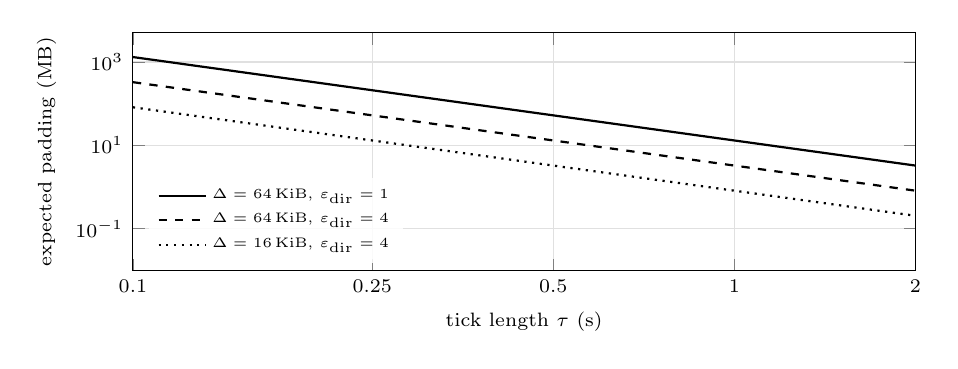
\begin{tikzpicture}
\begin{loglogaxis}[
  width=0.95\columnwidth, height=4.6cm,
  xlabel={tick length $\tau$ (s)}, ylabel={expected padding (MB)},
  xmin=0.1, xmax=2, ymin=0.01, ymax=5000,
  xtick={0.1,0.25,0.5,1,2}, xticklabels={0.1,0.25,0.5,1,2},
  legend style={font=\tiny, at={(0.02,0.03)}, anchor=south west, draw=none, fill=white, fill opacity=0.85, text opacity=1},
  tick label style={font=\scriptsize}, label style={font=\scriptsize},
  grid=major, grid style={black!12}, domain=0.1:2, samples=60]
\addplot[thick, solid] {20^2*65536/(2*x^2*1)/1e6};
\addlegendentry{$\Delta=64$\,KiB, $\varepsilon_{\mathrm{dir}}=1$}
\addplot[thick, dashed] {20^2*65536/(2*x^2*4)/1e6};
\addlegendentry{$\Delta=64$\,KiB, $\varepsilon_{\mathrm{dir}}=4$}
\addplot[thick, dotted] {20^2*16384/(2*x^2*4)/1e6};
\addlegendentry{$\Delta=16$\,KiB, $\varepsilon_{\mathrm{dir}}=4$}
\end{loglogaxis}
\end{tikzpicture}

\caption{Expected padding of the queue-length DP release per link-direction and session over a horizon $H=20$\,s, from \cref{eq:dpcost}, as a function of the tick length $\tau$, for two adjacency bounds $\Delta$ and per-direction budgets $\varepsilon_{\mathrm{dir}}$. Computed from the closed form, not measured. Plotted with PGFPlots from code prepared with AI assistance (Claude, Anthropic; see the generative AI declaration).}
\label{fig:dpcost}
\end{figure}

\begin{remark}[The exponent depends on the mechanism]\label{rem:exponent}
The quadratic growth belongs to the queue-length release with Laplace noise and basic composition, in which every tick is charged the full $\Delta$. Gaussian noise with R\'enyi DP accounting, as in NetShaper~\cite{sabzi2024netshaper}, gives, for a fixed total budget, a per-tick noise scale growing roughly like $\sqrt{K}$ (up to factors in $\log(1/\delta)$) and padding of order $K^{3/2}$. Releasing noisy \emph{arrivals} instead, $b_k=\max(0,\operatorname{round}(a_k+\mu+L_k))$ with $L_k\sim\mathrm{Lap}(\Delta/\varepsilon_{\mathrm{dir}})$ and a bias $\mu\ge0$, is $\varepsilon_{\mathrm{dir}}$-DP for the whole sequence by the Laplace mechanism on a vector with $\ell_1$ sensitivity $\Delta$; the padding per tick is at most $\max(0,\mu+L_k)$ plus half a byte, so total padding grows linearly in $K$, but the backlog is no longer bounded by the mechanism. Both variants are implemented; the completed resource evaluation uses the arrival variant and does not empirically compare the two privacy mechanisms.
\end{remark}

\begin{proposition}[Finite-horizon completion limit]\label{prop:completion}
Suppose $V\ge1$ integer bytes enter a link-direction only in its last tick, with no earlier real backlog. If the last release is $b=\max(0,\operatorname{round}(V+\mu+L))$, where $\mu\ge0$ is finite and $L\sim\mathrm{Lap}(0,s)$ with $s>0$, then
\[
 \Pr[\text{overflow}]=\tfrac12\exp\!\left(-\frac{\mu+1/2}{s}\right)>0.
\]
Thus neither finite bias in the arrivals mechanism nor the unbiased queue mechanism provides a universal zero-overflow guarantee under a fixed finite schedule that admits such arrivals.
\end{proposition}
\begin{proof}
No earlier release can serve bytes that have not arrived. The last release completes the input exactly when $b\ge V$. Apart from a probability-zero rounding tie, its complement is $L<-\mu-1/2$. The negative Laplace tail has the stated probability. Clipping at zero does not alter this event because $V\ge1$.
\end{proof}
This is a completion limit, not a refutation of the conditional release privacy statements. A deployment must declare its admissible arrivals and treatment of residual backlog; extra data-dependent sends after the horizon are outside the fixed-schedule guarantee. Empirical zero failures in a small pilot do not establish a hard reliability bound. The mechanism stress tests in \cref{sec:stress} examine this limit separately from real-network acquisition.

\begin{proposition}[Public-contract completion bound]\label{prop:contract}
On direction $j$, let integer arrivals have public total cap $V_j$, per-tick cap $A_j\le V_j$ and at most $M_j$ occupied ticks among $K_j$. They precede their tick's independent noise and arrive before the final release. In the arrivals mechanism use scale $s_j=\Delta_j/\varepsilon_j$ and finite bias $\mu_j\ge0$, optionally clipping every release to a fixed public $C_j\ge A_j$. Then
\[
 \Pr[\text{any residual backlog}]\le\sum_j\frac{M_j}{2}
       e^{-(\mu_j+1/2)/s_j}.
\]
For public $\rho_j>0$ with $\sum_j\rho_j\le\rho$, it suffices to set
\[
 \mu_j=\max\{0,s_j\log(M_j/(2\rho_j))-1/2\}.
\]
The expected application-byte release is at most
\[
 U_j=V_j+K_j\bigl[\mu_j+(s_j/2)e^{-\mu_j/s_j}+1/2\bigr],
\]
and with clipping is also bounded deterministically by $K_jC_j$.
\end{proposition}
\begin{proof}
At an occupied predictable tick, releasing fewer than its arrivals has conditional probability $p_j=\tfrac12 e^{-(\mu_j+1/2)/s_j}$. Public clipping above the arrival cap does not change this event. If it never occurs, induction leaves zero backlog after every tick. A union bound and the pathwise occupied-tick limit give $M_jp_j$ per direction, including arrivals adapted to past releases; union over directions gives the result. Also $\max(0,a+\mu+L)\le a+\max(0,\mu+L)$ for $a\ge0$, and rounding adds at most half a byte per tick. Taking expectations and summing proves $U_j$.
\end{proof}
Here $\rho$ bounds completion failure under the public arrival contract; it is not the $\delta$ of approximate DP and does not certify observable retries or aborts. Fixed clipping is output post-processing, not resampling truncated noise. The fixed-history adjacency assumptions still apply. The occupied-tick bound must be enforced at enqueue time: a streamed tool response may occupy several ticks, so counting tool calls alone is insufficient. Whole-message buffering or another justified bound is required. Late production outside the horizon remains a contract violation.

\begin{proposition}[Order of primitives]\label{prop:order}
If padding \cref{eq:pad} is applied before the DP release and the hypotheses differ in at most $n$ messages with total size at most $\Delta_0$, the padded arrival sequences differ by at most $r\Delta_0+n(\beta+1)$ bytes in $\ell_1$, so \cref{prop:dp} holds with $\Delta\ge r\Delta_0+n(\beta+1)$. If padding is applied to the released sequence instead, the guarantee of \cref{prop:dp} is unchanged and the padding adds bytes without reducing $\varepsilon$.
\end{proposition}
\begin{proof}
By \cref{prop:pad}(a) and the case $m\le\beta$, $\mathrm{pad}(m)\le\max(\beta,rm)+1\le\beta+rm+1$, where the $+1$ covers rounding to whole bytes; summing over the $n$ differing messages gives the bound. Padding the output is post-processing.
\end{proof}
The controller therefore applies rounds, then padding, then the DP release, and measures $\Delta$ directly on the bytes that enter the DP release in its calibration sessions, which satisfies \cref{prop:order} by construction.
